%!TEX root = ../thesis.tex
%*******************************************************************************
%*********************************** First Chapter *****************************
%*******************************************************************************

\chapter{PENDAHULUAN}  %Title of the First Chapter

	\ifpdf
	\graphicspath{{Chapter1/Figs/Raster/}{Chapter1/Figs/PDF/}{Chapter1/Figs/}}
	\else
	\graphicspath{{Chapter1/Figs/Vector/}{Chapter1/Figs/}}
	\fi


%********************************** %First Section  **************************************
\section{Latar Belakang}
 \textit{Breathing Rate} (BR) adalah salah satu indikator tanda vital utama, dan sering digunakan untuk menyimpulkan status kesehatan kardiopulmonari subjek.~Sebagai contoh, tingkat pernapasan yang lebih tinggi dari 27 kali per menit adalah prediktor paling penting untuk pasien serangan jantung [\citet{fieselmann1993}].~Berdasarkan \citet{Ganong}, rata-rata tingkat pernapasan (BR) pada orang dewasa berkisar antara 12-18 kali per menit.~Kombinasi detak jantung atau \textit{Heart Rate} (HR) dan tingkat pernapasan (BR) yang tinggi, tekanan darah sistolik rendah dan penurunan skor \textit{Glasgow Coma Scale} (GCS) adalah prediktor spesifik dari serangan jantung, masuk ICU yang tidak direncanakan dan kematian yang tidak terduga.~Selanjutnya ditemukan bahwa kasus tersebut dapat diidentifikasi hingga 24 jam sebelum kejadian [\citet{cretikos2007}].~Berdasarkan data Badan Penelitian \citep{RI2013} dalam Gambar~\ref{fig:data_penyakit_jantung} hal tersebut akan menguntungkan pasien karena segera mendapatkan penanganan dini.
\begin{figure}[ht]
	\vspace{0.5em}
	\centering
	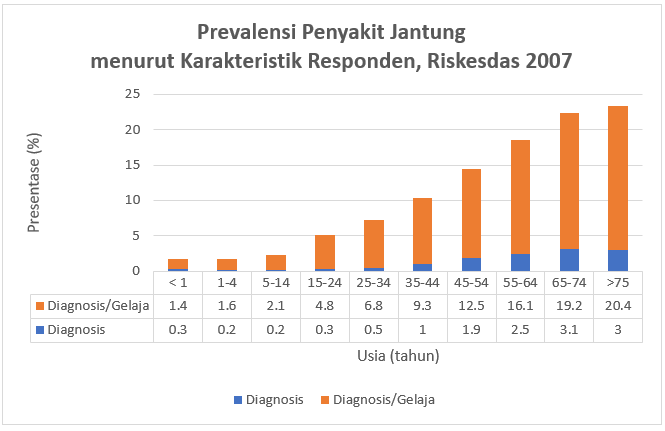
\includegraphics[width=0.7\textwidth]{Chapter1/Figs/chart_penderita_jantung}
	\caption{Data Penderita Penyakit Jantung Berdasarkan Rentan Usia Tahun 2007}
	\captionsetup{font={footnotesize}}
	\caption*{Sumber: Penelitian, B., 2013. Riset kesehatan dasar. Jakarta: Kementerian Kesehatan RI, halaman 116.}
	\label{fig:data_penyakit_jantung}   
\end{figure}

Pada pasien yang tidak stabil, perubahan tingkat BR relatif jauh lebih tinggi daripada perubahan nilai HR atau tekanan darah sistolik, dan dengan demikian tingkat pernapasan kemungkinan menjadi cara yang lebih baik untuk membedakan antara pasien yang stabil dan tidak [\citet{subbe2003}].~Namun, dalam kebanyakan kasus, informasi tentang HR dan BR akan mampu menunjukkan diagnosa yang lebih baik.~Oleh karena itu, dalam penelitian ini sangat penting untuk mendapatkan pengukuran pasien  baik dari jantung maupun napas.

\begin{figure}[ht]
	\vspace{0.5em}
	\centering
	\begin{subfigure}[b]{0.47\textwidth}
		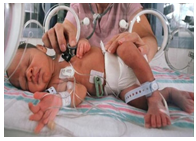
\includegraphics[width=\textwidth]{Chapter1/Figs/baby}
		\caption{}
	\end{subfigure}             
	\begin{subfigure}[b]{0.47\textwidth}
		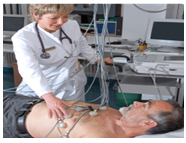
\includegraphics[width=\textwidth]{Chapter1/Figs/adult}
		\caption{}
	\end{subfigure}
	\caption[Proses monitor detak jantung dan pernapasan pada bayi (a) dan orang dewasa (b)]{Proses monitor detak jantung dan pernapasan pada bayi (a) dan orang dewasa (b).~Terlihat terlalu banyak selang-selang sensor yang membuat pasien tidak nyaman yang mengakibatkan posisi sensor mudah bergeser karena gerakan pasien, ataupun secara sengaja oleh pasien, khususnya pada bayi.}
	\captionsetup{font={footnotesize}}
	\caption*{Sumber: (a) https://www.bbc.com/news/health-30034760 (b) http://www.heart.org/HEARTORG/\\Conditions/HeartFailure/DiagnosingHeartFailure/Common-Tests-for-Heart-
		Failure\_UCM\_306334\_Article.jsp (diakses tanggal 6 Juni 2018)}
	\label{fig:pengukuran_jantung}
\end{figure}

Penelitian sebelumnya telah diajukan dalam literatur [\citet{kristjansdottir2004,leonard2006,nilsson2000,nam2014,tarrant1997}] untuk memperkirakan nilai HR dan BR.~Metode yang paling umum untuk mengukur HR dan BR adalah menghitung secara manual pergerakan jantung, dan dinding dada atau suara napas dengan stetoskop.~Namun, penelitian sebelumnya telah menunjukkan bahwa metode manual ini cenderung tidak dapat diandalkan dalam perawatan pasien akut, dan dibatasi oleh keahlian pengukuran dokter [\citet{hillman2005}].~Untuk proses monitor melalui penggunaan sensor-sensor seperti \textit{Respiratory Inductance Plethysmography} (RIP), oximeter, pengukur regangan atau magnetometer telah digunakan pada penelitian-penelitian sebelumnya  [\citet{Mendelson2006,Renevey2001,tarrant1997,Yang1998}].~Photoplethysmography (PPG) juga telah banyak digunakan untuk memperkirakan tingkat pernapasan karena kesederhanaan [\citet{Allen2007,Kamal1989,kristjansdottir2004}].~Namun, penggunaan sensor-sensor untuk monitor HR dan BR dalam praktisnya sulit untuk diterapkan karena pasien cenderung merasa tidak nyaman ---khususnya pada bayi, seperti pada Gambar~\ref{fig:pengukuran_jantung}--- dan mudah mengubah posisi sensor yang berakibat pada ketidak-akuratan pengukuran.

Penelitian sebelumnya yang menggunakan \textit{non-wearable} sensor seperti kamera yaitu oleh [\citet{lazaro2014,nam2014}].~Dengan menggunakan kamera misalnya smartphone atau kamera infrared untuk memonitor HR dan BR hanya pada bagian tubuh tertentu misalnya kepala ataupun warna kulit kepala.~Dalam praktisnya hal ini sulit untuk diterapkan karena metode tersebut hanya khusus untuk karakteristik bagian tubuh tertentu, dan penempatan posisi kamera terlihat kurang praktis karena menggunakan kamera sejenis smartphone.
%********************************** %Second Section  *************************************
\section{Tujuan Proyek Akhir} %Section - 1.2

Tujuan utama dari proyek akhir ini adalah mengembangkan sistem monitoring detak jantung (HR) dan pernapasan (BR) secara real-time berbasis \textit{non-wearable vision} ---menggunakan sensor yang \textit{non-wearable} berupa kamera yang tidak perlu dipasangkan langsung pada pasien---.~Sistem monitoring yang dirancang tidak hanya terbatas pada bagian tubuh tertentu, namun bisa pada bagian tubuh yang lain yang menunjukkan adanya aktifitas jantung maupun pernapasan, misalnya denyut jantung pada nadi pergelangan tangan, perut, leher, dan kepala.~Dengan demikian diyakini penempatan kamera akan menjadi lebih praktis misalnya dengan memanfaatkan kamera CCTV yang sudah tersedia di masing-masing kamar pasien.
Hipotesa penelitian ini adalah dengan menganalisa pergerakan piksel-piksel (RGB) pada area tubuh yang akan dimonitor HR dan BR-nya, akan didapatkan amplitudo dan frekuensi pergerakan piksel-piksel tersebut.~Frekuensi dan amplitudo tertentu yang tidak kasat mata akan menggambarkan gerakan tertentu pada manusia seperti detak jantung, pernapasan, kedip mata, atau bahkan aliran darah.~Piksel-piksel tersebut akan ditambahkan filter sesuai frekuensi dan amplitudonya yang kemudian akan dikuatkan seperti halnya penguatan sinyal pada audio.

%********************************** % Third Section  *************************************
\section{Rumusan Masalah}  %Section - 1.3 
%\label{section1.3}

Monitoring HR dan BR yang \textit{non-wearable} ---tanpa pemasangan sensor pada tubuh pasien--- sangat penting dan dibutuhkan.~Pemasangan sensor-sensor pada bagian tubuh cenderung membuat tidak nyaman, dan rentan lepas atau bergeser baik itu secara sengaja ataupun tidak sengaja oleh pasien, hal ini terjadi khususnya pada bayi.~Oleh karena itu, penggunaan \textit{non-wearable} sensor seperti kamera menarik untuk diteliti lebih lanjut.

Penelitian sebelumnya dengan menggunakan kamera [\citet{lazaro2014,nam2014}] cenderung fokus hanya pada bagian tubuh tertentu untuk monitor jantung dan pernapasan.~Metode tertentu hanya dapat bekerja untuk bagian tubuh tertentu tetapi tidak untuk bagian tubuh lain.~Ditambah dengan penggunaan kamera smartphone yang mengakibatkan kurang praktis untuk penempatan posisi kamera, misalnya di rumah sakit.~Dari penjelasan sebelumnya, permasalahan yang akan dibahas dalam penelitian ini yaitu:
\begin{enumerate}
\item Apakah perbedaan pengukuran HR dan BR menggunakan metode \textit{wearable} dan \textit{non-wearable}?
\item Bagaimana proses monitoring HR dan BR menggunakan metode \textit{non-wearable}?
\item Bagaimana melakukan pengukuran HR dan BR pada bagian tubuh yang berbeda dengan menggunakan kamera?
\end{enumerate}


%********************************** % Forth Section  *************************************
\section{Batasan Masalah}  %Section - 1.4

Dari rumusan masalah tersebut, akan dilakukan batasan masalah yaitu:
\begin{enumerate}
	\item Pembahasan hanya mengenai proses pengolahan gambar.
	\item Monitoring dilakukan pada bagian tubuh yang menunjukkan adanya aktifitas jantung maupun pernapasan (pergelangan tangan, leher, perut dan kepala).
	\item Uji coba dilakukan pada pencahayaan yang cukup.
	\item Jarak monitoring yang terbatas.
	\item Jumlah kamera yang digunakan satu.
	\item Posisi kamera konstan.
	\item Monitoring dilakukan selama adanya perubahan piksel.
	
\end{enumerate}

%********************************** % Fifth Section  *************************************
\section{Metodologi Proyek Akhir}  %Section - 1.5 
Metodologi yang digunakan pada penelitian tugas akhir ini adalah sebagai berikut:
\newline
\begin{enumerate}
	\item Studi Literatur
	\begin{itemize}
		\item Mencari dan mempelajari karakterisitik dan mekanisme sistem pernapasan dan detak jantung pada manusia.
		\item Mencari dan mempelajari \textit{Digital Signal Processing}.
		\item Mencari dan mengumpulkan dataset HR dan BR.
	\end{itemize}
	\item Implementasi metode untuk monitoring HR dan BR
	\begin{itemize}
		\item Proses ekstraksi sinyal HR dan BR dari bagian tubuh yang telah ditentukan.
		\item Mengolah sinyal HR dan BR yang diperoleh menjadi nilai eksak.
	\end{itemize}
	\item Implementasi program 
	Berdasarkan hasil monitoring yang didapatkan sebelumnya, kemudian dibuat progam dengan \textit{User Interface} dan diaplikasikan pada hardware yang telah ditentukan untuk proses monitoring secara real time. 
	\item Proses pembuatan \textit{User Interface} program dan komunikasi serial interface.
	\item Desain \textit{casing} hardware.
	\item Pengujian dan Analisa Data.
	\begin{itemize}
		\item Membahas mengenai pengujian metode dan \textit{User Interface} program dari sistem monitoring HR dan BR. 
		\item Melakukan analisa dari metode dan \textit{User Interface} program yang telah dicapai hingga saat pengujian.
	\end{itemize}
\end{enumerate}

%********************************** % Sixth Section  *************************************
\section{Sistematika Penulisan}  %Section - 1.6 

Sistematika penulisan berisi tentang bagaimana menyajikan laporan proyek akhir.~Sistematika yang akan diuraikan dalam proposal proyek akhir ini terbagi dalam BAB-BAB yang akan dibahas sebagai berikut:

BAB 1: PENDAHULUAN

Berisi latar belakang pembuatan proyek akhir, rumusan masalah dalam proyek akhir ini, batasan masalah, tujuan dari rumusan masalah, luaran yang diharapkan, metedologi untuk menyelesaikan proyek akhir ini, dan sistematika penulisan.

BAB 2: STUDI PUSTAKA

Berisi tentang tinjauan pustaka penelitian sebelumnya dan teori penunjang yang mendukung dalam perencanaan serta pembuatan proyek akhir ini.~Teori yang ditinjau mengacu pada penelitian-penelitian sebelumnya tentang macam-macam penelitian tentang pengukuran HR dan BR, penelitian \textit{Photoplethysmography}, dan penggunaan \textit{Digital Image Processing} serta \textit{Digital Signal Processing}.

BAB 3: PERANCANGAN DAN PEMBUATAN SISTEM

Berisi tentang gambaran umum sistem yang akan dibangun, desain perancangan komputer, hardware dan komunikasi yang digunakan, serta pembuatan \textit{User Interface} program.

BAB 4: PENGUJIAN DAN ANALISA SISTEM

Berisi tentang pengujian dari masing-masing bagian sistem dan pengujian sistem sementara.~Pada BAB ini akan diperlihatkan hasil yang telah diterapkan dan pada bagian mana dapat dilakukan penyempurnaan.

BAB 5: PENUTUP

Berisi kesimpulan dan analisa sistem dari proyek akhir yang telah didapat serta saran-saran untuk pengembangan selanjutnya.